\documentclass{template/socthesis}

\usepackage{subcaption} 
\usepackage{amsmath} 
\usepackage{enumitem} 
\usepackage{hyperref} % reference
\usepackage{gensymb} % balíček symbolů
\usepackage{booktabs}

\usepackage[toc,page]{appendix}
\usepackage{color} % balíček pro obarvování textů
\usepackage{xcolor}  % zapne možnost používání barev, mj. pro \definecolor
\definecolor{mygreen}{RGB}{0,150,0} % nastavení barev odkazů 
\usepackage{listings} % balíček pro formátování zdrojových kódů 
\usepackage{multirow}
\usepackage{pifont}
\usepackage[author=,status=draft]{fixme} % vkládání poznámek  
% dva módy (status): draft (poznámky se zobrazují v PDF) / final (poznámky se nezobrazují v PDF)

\newcommand{\cmark}{\textcolor{green}{\ding{51}}}%
\newcommand{\xmark}{\textcolor{red}{\ding{55}}}%

\lstset { %
    language=C++,
    backgroundcolor=\color{black!5}, % set backgroundcolor
    basicstyle=\footnotesize,% basic font setting
}

\addbibresource{text.bib} % soubor s bibliografií
\nocite{*}

\titlecz{Integrace do průmyslu 4.0} % český název práce
\titleen{Integration into industry 4.0} % anglický název práce
\author{Jakub Andrýsek} % jméno a příjmení autora
\field{18} % obor (pouze číslo, zbytek vysází šablona - číslo oboru viz http://www.soc.cz/obory-soc/)
\school{Gymnázium Brno, Vídeňská, příspěvková organizace} % celý název školy
\mentor{Mgr. Jaroslav Páral} % jméno a příjmení školitele
\mentorstatement{Mgr. Jaroslava Párala} % jméno a příjmení ve druhém pádě 

% Změňte, pokud se liší
%\region{Jihomoravský} % kraj
\placefooter{Brno 2021} % místo a rok

% hinty k používání balíčků hyperref, url, hyperlink a hypertarget
% \usepackage{hyperref} % balíček pro hypertextové odkazy
% \url{www.odkaz.cz}
% \href{http://www.odkaz.cz}{Text který bude jako odkaz}
% \hyperlink{label}{proklikávací_text} - odkaz na text 
% \hypertarget{label}{cíl_odkazu} - cíl odkazu 

\begin{document} % konec preambule dokumentu

\maketitle % vysází titulky

\makecopyrightstatement{V~Brně} % místo

% poděkování
\makethanks{Děkuji svému školiteli Mgr. Jaroslavovi Páralovi za obětavou pomoc, podnětné připomínky a~hlavně nekonečnou trpělivost, kterou mi během práce poskytoval.}

\pagestyle{empty}

\section*{Anotace}
\color{mygreen}
Anotace má za úkol stručně popsat cíle práce a velmi stručný úvod k tématu. 
Většinou bývá použit první odstavec, nebo jiná část úvodu.
\color{black}

Zahradničení je dnes naprosto běžnou zájmovou činností. Mnoho lidí mající takovou zálibu je ovšem velmi časově vytížených. Kromě práce se musí starat mnohdy i o~rodinu a~na péči o~rostliny jim často jednoduše nezbývá čas. Jedním z~těchto lidí je i můj táta, který mě inspiroval k~vytvoření PROTOPlantu -- systému pro snadnou a~levnou automatizaci skleníku. 

Cílem práce je vytvořit univerzální a~dostupný systém pro automatizaci skleníku, který by usnadnil péči o~rostliny časově vytíženým lidem. 

\subsection*{Klíčová slova}
\color{mygreen}
Klíčová slova.
Snažte se najít alespoň 5, ideálně i více klíčových slov, která jednoduše vystihují vaši práci.
\color{black}

automatizace skleníku, ESP32, PROTOPlant, automatizace, open-source hardware, open-source software

\newpage % pokud se anotace vleze na jednu stránku (což by měla), tento rádek zakomentuj

\vspace{20mm}

\section*{Annotation}
\color{mygreen}
Zde přijde anglický překlad anotace.
\color{black}

Gardening is a~very common hobby today. However, many people who likes this activity doesn't have enough time for it. 
Beside work, they have to take care of their families and after this, they don't have any time to take care of plants. 
My dad is exactly this kind of man. 
And that inspired me to create PROTOPlant -- system for easy and cheap greenhouse automation.

Goal of this thesis is to create universal and available system for greenhouse automation, that will make it easier for these people to take care of their plants.

\subsection*{Keywords}
\color{mygreen}
Klíčová slova - jejich překlad do angličtiny.
\color{black}

greenhouse automation, ESP32, PROTOPlant, automation, open-source hardware, open-source software

\newpage
\pagestyle{plain}

\tableofcontents % vysází obsah

%%% Začátek práce
\setcounter{figure}{0}
\setcounter{table}{0}
\newpage

% zde můžeš s pomocí příkazu \input{cesta k souboru} vložit soubory; doporučuji každou větší kapitolu dát do samostatného souboru pro větší přehlednost

% Úvod práce
\chapter*{Úvod}
\addcontentsline{toc}{chapter}{Úvod}
Cílem práce je navrhnout ucelený systém monitorující chod pletacích strojů ve firmě a~přizpůsobit ho co možná nejlépe potřebám firmy.

S~nápadem vytvořit takovýto systém přišel můj děda, zakladatel firmy na výrobu ponožek.
Jeho snem vždy bylo mít takový systém, který by částečně zastal monotónní lidskou práci a~nahradil ji efektivní automatizací.

Můj systém jsem tedy navrhoval na míru pro rodinnou firmu na pletení ponožek, ve které je okolo 25 pletacích strojů. 
Tento systém je schopen v~reálném čase zaznamenávat a~následně odesílat naměřená data ze strojů na server. 
Pro uživatele pak systém nabízí moderní webové stránky, kde si může naměřená data přehledně zobrazit a~analyzovat.

Podle pletacích strojů na kterých tento systém běží jsem projekt pojmenoval Pletačka IoT. 
Systém se skládá ze tří částí. Senzorová část, která je připojená k~pletacímu stroji a~odesílá data.
Dále pak server, který veškerá data zpracovává a~zobrazuje je uživateli.
Poslední částí je podpůrný server, který se stará o~aktualizaci a~o~kontrolu správného chodu senzorů.\newline


Při~vytváření tohoto projektu jsem si dal za cíl
\begin{itemize}
    \item projekt s~otevřeným zdrojovým kódem
    \item cenová dostupnost
    \item jednoduché přidání senzorů
    \item přehledné uživatelské rozhraní
\end{itemize}

Pro systém jsem si stanovil tyto požadavky
\begin{itemize}
    \item Počítání upletených ponožek
    \item Zjišťování poruchovosti strojů
    \item Porovnání jednotlivých pracovních směn
    \item Monitorování průběhu výroby
\end{itemize}

\newpage



\chapter{Konkurence}
Lorem ipsum dolor sit amet, consectetur adipiscing elit.
Aliquam nunc magna, sollicitudin id leo eu, viverra congue risus.
Aliquam consequat ipsum ut erat placerat consequat nec at diam. 
Aenean est odio, molestie sit amet nunc in, pretium luctus elit. 
Donec imperdiet orci vel porttitor placerat. 
Proin ut hendrerit elit, ultricies accumsan urna. 
Vivamus condimentum lorem viverra lectus finibus, nec volutpat turpis auctor.
Cras quis felis non lorem consectetur interdum eu eu sem. 
Proin sit amet feugiat metus. 
Ut vitae orci a enim vestibulum porta:
\begin{itemize} % odrážkový seznam
    \item lorem
    \item ipsum
    \item lorem ipsum
    \item lipsum
\end{itemize}

\begin{table}[h]
    \centering
    \resizebox{\textwidth}{!}{%
    \begin{tabular}{@{}l|lll@{}}
        & \textbf{Průmyslová řešení} & \textbf{„Kutilská“ řešení} & \textbf{PROTOPlant}                                                                                   \\ \midrule
    \textbf{Dodání}      & Výroba na zakázku          & „Vyrob si sám“             & \begin{tabular}[c]{@{}l@{}}Možnost sestavení přímo doma, \\ nebo dodání \B{hotového} systému\end{tabular} \\
    \textbf{Cena}        & Drahá ($>$~10~000~Kč)      & Levná ($<$~10~000~Kč)      & Kompromis cena -- výkon (již od 2~500~Kč)                                                                               \\
    \textbf{Ovládání}    & Komplexní                  & Jednoduché (většinou)      & Jednoduché                                                                                            \\
    \textbf{Konektivita} & Většinou ethernet          & Často Wi-Fi                & \begin{tabular}[c]{@{}l@{}}Wi-Fi, Bluetooth, \\ možnost přidání podpory Ethernetu\end{tabular}        \\
    \textbf{Řízení}      & PLC                        & Většinou Arduino           & ESP32                                                                                                 \\ \bottomrule
    \textbf{Modularita}  & Ano                        & Ne                         & Ano                                                                                                   \\
    \textbf{Univerzálnost}& Ano                       & Ne                         & Ano                                                                                                   \\ 
    \textbf{Open-source} & Ne                         & Většinou ano               & Ano                                                                                                   \\ \bottomrule    
    \end{tabular}%
    }
    \caption{Tabulka srovnání PROTOPlantu a~jiných řešení.}
    \label{tab:COMPARATION}
\end{table}

\begin{figure}[htbp]
    \centering
    \includegraphics[width=\textwidth]{img/I2C.png}
    \caption{Celý datový přenos po I2C sběrnici. Převzato z~\cite{I2C_specs}}
    \label{fig:I2C-protocol}
 \end{figure}
 
\noindent\B{Lipsum} -- lorem ipsum dolor sit amet, consectetur adipiscing elit.
Aliquam nunc magna, sollicitudin id leo eu, viverra congue risus.
Aliquam consequat ipsum ut erat placerat consequat nec at diam. 
Aenean est odio, molestie sit amet nunc in, pretium luctus elit. 
Donec imperdiet orci vel porttitor placerat. 
Proin ut hendrerit elit, ultricies accumsan urna. 
Vivamus condimentum lorem viverra lectus finibus, nec volutpat turpis auctor.
Cras quis felis non lorem consectetur interdum eu eu sem. 
Proin sit amet feugiat metus. 
Ut vitae orci a enim vestibulum porta. \newline

\section{Sumarizace}
Nabídka řešení v~tomto oboru je velmi chudá.
Na jedné straně stojí průmyslová řešení, která jsou drahá a~dodávají se primárně do skleníků velkých zemědělských firem.
Na opačném břehu jsou řešení amatérská. 
Ta jsou ovšem buďto naprosto nepoužitelná v~běžně velkém skleníku (primárně je uživatelé vyrábí pro malá pařeniště), nebo neuniverzální.

\newpage


\chapter{Integrace do průmyslu 4.0}
Pojem Průmysl 4.0 se do České republiky dostal okolo roku 2013 a~od té doby se stále více rozšiřuje v~průmyslových firmách.
Jedna z~klíčových částí je IoT (Internet of Things), neboli v~internet věcí, který nám zajišťuje vzdálenou kontrolu a~řízení strojů pomocí elektroniky, senzorů a~různých softwarů.
Další vlastností těchto systémů je zaznamenávání a~následné ukládání dat do datových úložišť.
Moderní IoT řídící systémy se snaží proniknou co nejvíce do hloubky řídících systém a~zpřesnit tak naměřená data, důležitá pro optimalizaci produkce.   

%SECTION
\section{Popis}
Při~návrhu mého systému jsem se snažil řídit těmito zásadami a~navrhnout tak co nejmodernější a~provozně efektivní systém.
Základem bylo zhodnocení stávající situace a~navržení možného řešení.

Jednotlivé problémy
\begin{itemize}
    \item dlouhá doba stání nečinných strojů při poruše i nedostatku materiálu
    \item ruční počítání vyprodukovaného zboží
    \item absence historického přehledu produkce
\end{itemize}

%SECTION
\section{Řešení}
Mým řešením je tedy návrh moderního systému, který by celý tento provoz monitoroval a~zobrazoval zaměstnavateli.
Dále se také snažím o~zhodnocení jednotlivých směn a~jejich porovnání.
Systém neustále vyvíjím a~rozšiřuji podle potřeb firmy.

Funkce systému
\begin{itemize}
    \item monitoring provozu firmy
    \item porovnání pracovních směn
    \item počítání upletených ponožek
\end{itemize}



%SECTION
\section{Nasazení}
Tento systém je aktuálně nasazen ve firmě ROTEX Vysočina s.r.o\cite{ROTEX}, která se věnuje výrobě ponožek. 
Firma pracuje ve dvousměnném provozu a~týdně vyprodukuje v~průměru 12000 párů ponožek. 

Díky mému systému by se ve firmě dala optimalizovat produkce a~výkon strojů a~tím zefektivnit budoucí výrobu. 



%SECTION
\section{Pletací stroj}



\begin{figure}[htbp]
    \centering
    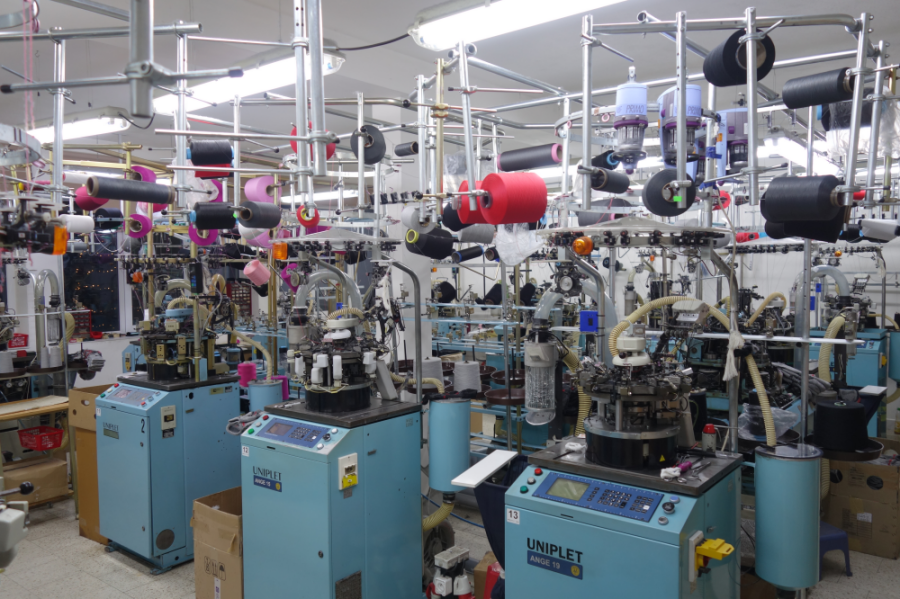
\includegraphics[width=\textwidth]{img/pletarna.png}
    \caption{Pletárna ponožek}
    \label{fig:Pletarna}
\end{figure}

\begin{figure}[htbp]
    \centering
    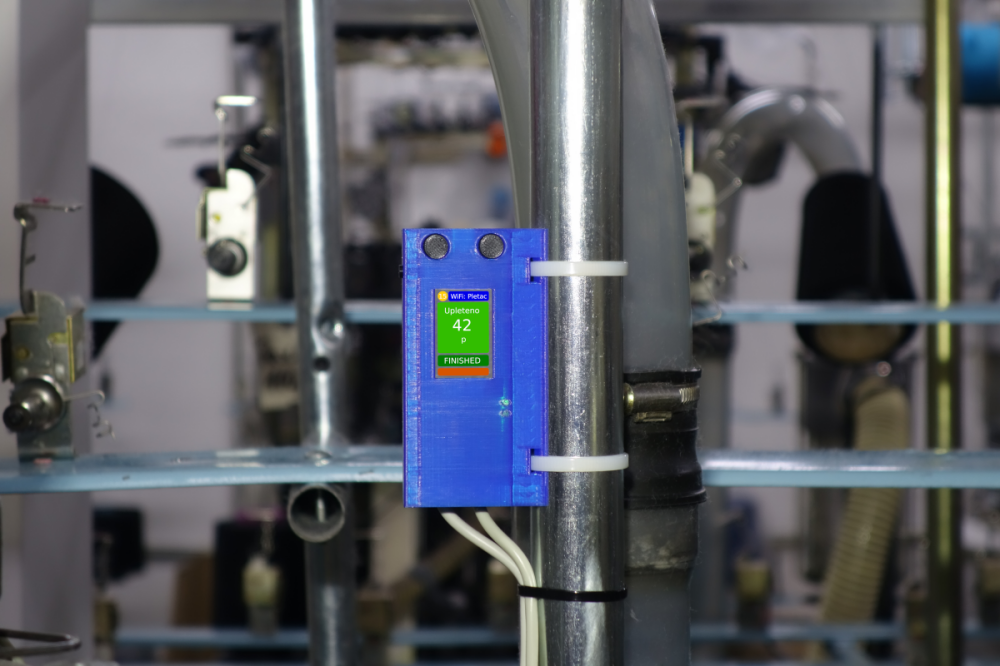
\includegraphics[width=\textwidth]{img/V2-uchyceni.png}
    \caption{Senzor na stroji}
    \label{fig:SenzorNaStroji}
\end{figure}


\newpage


% \chapter{Systém Pletačka-IoT}


% %SECTION
% \section{Popis}
% Lorem ipsum dolor sit amet, consectetur adipiscing elit.
% Aliquam nunc magna, sollicitudin id leo eu, viverra congue risus.
% Aliquam consequat ipsum ut erat placerat consequat nec at diam. 
% Aenean est odio, molestie sit amet nunc in, pretium luctus elit. 
% Donec imperdiet orci vel porttitor placerat. 
% Proin ut hendrerit elit, ultricies accumsan urna. 
% Vivamus condimentum lorem viverra lectus finibus, nec volutpat turpis auctor.
% Cras quis felis non lorem consectetur interdum eu eu sem. 
% Proin sit amet feugiat metus. 
% Ut vitae orci a enim vestibulum porta. 

% %SECTION
% \section{Využití}
% Lorem ipsum dolor sit amet, consectetur adipiscing elit.
% Aliquam nunc magna, sollicitudin id leo eu, viverra congue risus.
% Aliquam consequat ipsum ut erat placerat consequat nec at diam. 
% Aenean est odio, molestie sit amet nunc in, pretium luctus elit. 
% Donec imperdiet orci vel porttitor placerat. 
% Proin ut hendrerit elit, ultricies accumsan urna. 
% Vivamus condimentum lorem viverra lectus finibus, nec volutpat turpis auctor.
% Cras quis felis non lorem consectetur interdum eu eu sem. 
% Proin sit amet feugiat metus. 
% Ut vitae orci a enim vestibulum porta. 


% %SECTION
% \section{Naszaení}
% Lorem ipsum dolor sit amet, consectetur adipiscing elit.
% Aliquam nunc magna, sollicitudin id leo eu, viverra congue risus.
% Aliquam consequat ipsum ut erat placerat consequat nec at diam. 
% Aenean est odio, molestie sit amet nunc in, pretium luctus elit. 
% Donec imperdiet orci vel porttitor placerat. 
% Proin ut hendrerit elit, ultricies accumsan urna. 
% Vivamus condimentum lorem viverra lectus finibus, nec volutpat turpis auctor.
% Cras quis felis non lorem consectetur interdum eu eu sem. 
% Proin sit amet feugiat metus. 
% Ut vitae orci a enim vestibulum porta. 


% \newpage


\chapter{Senzory}
Lorem ipsum dolor sit amet, consectetur adipiscing elit.
Aliquam nunc magna, sollicitudin id leo eu, viverra congue risus.
Aliquam consequat ipsum ut erat placerat consequat nec at diam. 
Aenean est odio, molestie sit amet nunc in, pretium luctus elit. 
Donec imperdiet orci vel porttitor placerat. 
Proin ut hendrerit elit, ultricies accumsan urna. 
Vivamus condimentum lorem viverra lectus finibus, nec volutpat turpis auctor.
Cras quis felis non lorem consectetur interdum eu eu sem. 
Proin sit amet feugiat metus. 
Ut vitae orci a enim vestibulum porta. 



\section{Univerzální sensorika}
Lorem ipsum dolor sit amet, consectetur adipiscing elit.
Aliquam nunc magna, sollicitudin id leo eu, viverra congue risus.
Aliquam consequat ipsum ut erat placerat consequat nec at diam. 
Aenean est odio, molestie sit amet nunc in, pretium luctus elit. 
Donec imperdiet orci vel porttitor placerat. 
Proin ut hendrerit elit, ultricies accumsan urna. 
Vivamus condimentum lorem viverra lectus finibus, nec volutpat turpis auctor.
Cras quis felis non lorem consectetur interdum eu eu sem. 
Proin sit amet feugiat metus. 
Ut vitae orci a enim vestibulum porta. 


\subsection{Něco tu bude}
Lorem ipsum dolor sit amet, consectetur adipiscing elit.
Aliquam nunc magna, sollicitudin id leo eu, viverra congue risus.
Aliquam consequat ipsum ut erat placerat consequat nec at diam. 
Aenean est odio, molestie sit amet nunc in, pretium luctus elit. 
Donec imperdiet orci vel porttitor placerat. 
Proin ut hendrerit elit, ultricies accumsan urna. 
Vivamus condimentum lorem viverra lectus finibus, nec volutpat turpis auctor.
Cras quis felis non lorem consectetur interdum eu eu sem. 
Proin sit amet feugiat metus. 
Ut vitae orci a enim vestibulum porta. 


\newpage

\section{Speciální senzorika}
Lorem ipsum dolor sit amet, consectetur adipiscing elit.
Aliquam nunc magna, sollicitudin id leo eu, viverra congue risus.
Aliquam consequat ipsum ut erat placerat consequat nec at diam. 
Aenean est odio, molestie sit amet nunc in, pretium luctus elit. 
Donec imperdiet orci vel porttitor placerat. 
Proin ut hendrerit elit, ultricies accumsan urna. 
Vivamus condimentum lorem viverra lectus finibus, nec volutpat turpis auctor.
Cras quis felis non lorem consectetur interdum eu eu sem. 
Proin sit amet feugiat metus. 
Ut vitae orci a enim vestibulum porta. 


\subsection{Něco tu bude}
Lorem ipsum dolor sit amet, consectetur adipiscing elit.
Aliquam nunc magna, sollicitudin id leo eu, viverra congue risus.
Aliquam consequat ipsum ut erat placerat consequat nec at diam. 
Aenean est odio, molestie sit amet nunc in, pretium luctus elit. 
Donec imperdiet orci vel porttitor placerat. 
Proin ut hendrerit elit, ultricies accumsan urna. 
Vivamus condimentum lorem viverra lectus finibus, nec volutpat turpis auctor.
Cras quis felis non lorem consectetur interdum eu eu sem. 
Proin sit amet feugiat metus. 
Ut vitae orci a enim vestibulum porta. 



\newpage


\chapter{Webový server}
Lorem ipsum dolor sit amet, consectetur adipiscing elit.
Aliquam nunc magna, sollicitudin id leo eu, viverra congue risus.
Aliquam consequat ipsum ut erat placerat consequat nec at diam. 
Aenean est odio, molestie sit amet nunc in, pretium luctus elit. 
Donec imperdiet orci vel porttitor placerat. 
Proin ut hendrerit elit, ultricies accumsan urna. 
Vivamus condimentum lorem viverra lectus finibus, nec volutpat turpis auctor.
Cras quis felis non lorem consectetur interdum eu eu sem. 
Proin sit amet feugiat metus. 
Ut vitae orci a enim vestibulum porta. 

%SECTION
\section{Webový server}
Lorem ipsum dolor sit amet, consectetur adipiscing elit.
Aliquam nunc magna, sollicitudin id leo eu, viverra congue risus.
Aliquam consequat ipsum ut erat placerat consequat nec at diam. 
Aenean est odio, molestie sit amet nunc in, pretium luctus elit. 
Donec imperdiet orci vel porttitor placerat. 
Proin ut hendrerit elit, ultricies accumsan urna. 
Vivamus condimentum lorem viverra lectus finibus, nec volutpat turpis auctor.
Cras quis felis non lorem consectetur interdum eu eu sem. 
Proin sit amet feugiat metus. 
Ut vitae orci a enim vestibulum porta. 



%SECTION
\section{Funkcionalita}
Lorem ipsum dolor sit amet, consectetur adipiscing elit.
Aliquam nunc magna, sollicitudin id leo eu, viverra congue risus.
Aliquam consequat ipsum ut erat placerat consequat nec at diam. 
Aenean est odio, molestie sit amet nunc in, pretium luctus elit. 
Donec imperdiet orci vel porttitor placerat. 
Proin ut hendrerit elit, ultricies accumsan urna. 
Vivamus condimentum lorem viverra lectus finibus, nec volutpat turpis auctor.
Cras quis felis non lorem consectetur interdum eu eu sem. 
Proin sit amet feugiat metus. 
Ut vitae orci a enim vestibulum porta. 


%SECTION
\section{Fronted}
Lorem ipsum dolor sit amet, consectetur adipiscing elit.
Aliquam nunc magna, sollicitudin id leo eu, viverra congue risus.
Aliquam consequat ipsum ut erat placerat consequat nec at diam. 
Aenean est odio, molestie sit amet nunc in, pretium luctus elit. 
Donec imperdiet orci vel porttitor placerat. 
Proin ut hendrerit elit, ultricies accumsan urna. 
Vivamus condimentum lorem viverra lectus finibus, nec volutpat turpis auctor.
Cras quis felis non lorem consectetur interdum eu eu sem. 
Proin sit amet feugiat metus. 
Ut vitae orci a enim vestibulum porta. 


\subsection{Bootstrap}
Lorem ipsum dolor sit amet, consectetur adipiscing elit.
Aliquam nunc magna, sollicitudin id leo eu, viverra congue risus.
Aliquam consequat ipsum ut erat placerat consequat nec at diam. 
Aenean est odio, molestie sit amet nunc in, pretium luctus elit. 
Donec imperdiet orci vel porttitor placerat. 
Proin ut hendrerit elit, ultricies accumsan urna. 
Vivamus condimentum lorem viverra lectus finibus, nec volutpat turpis auctor.
Cras quis felis non lorem consectetur interdum eu eu sem. 
Proin sit amet feugiat metus. 
Ut vitae orci a enim vestibulum porta. 


\subsection{JavaScript}

!!!! Proč jsem zvolil tyto technologie, knihovny !!!!

Lorem ipsum dolor sit amet, consectetur adipiscing elit.
Aliquam nunc magna, sollicitudin id leo eu, viverra congue risus.
Aliquam consequat ipsum ut erat placerat consequat nec at diam. 
Aenean est odio, molestie sit amet nunc in, pretium luctus elit. 
Donec imperdiet orci vel porttitor placerat. 
Proin ut hendrerit elit, ultricies accumsan urna. 
Vivamus condimentum lorem viverra lectus finibus, nec volutpat turpis auctor.
Cras quis felis non lorem consectetur interdum eu eu sem. 
Proin sit amet feugiat metus. 
Ut vitae orci a enim vestibulum porta. 


%SECTION
\section{Backend}
Lorem ipsum dolor sit amet, consectetur adipiscing elit.
Aliquam nunc magna, sollicitudin id leo eu, viverra congue risus.
Aliquam consequat ipsum ut erat placerat consequat nec at diam. 
Aenean est odio, molestie sit amet nunc in, pretium luctus elit. 
Donec imperdiet orci vel porttitor placerat. 
Proin ut hendrerit elit, ultricies accumsan urna. 
Vivamus condimentum lorem viverra lectus finibus, nec volutpat turpis auctor.
Cras quis felis non lorem consectetur interdum eu eu sem. 
Proin sit amet feugiat metus. 
Ut vitae orci a enim vestibulum porta. 


\subsection{PHP}
Lorem ipsum dolor sit amet, consectetur adipiscing elit.
Aliquam nunc magna, sollicitudin id leo eu, viverra congue risus.
Aliquam consequat ipsum ut erat placerat consequat nec at diam. 
Aenean est odio, molestie sit amet nunc in, pretium luctus elit. 
Donec imperdiet orci vel porttitor placerat. 
Proin ut hendrerit elit, ultricies accumsan urna. 
Vivamus condimentum lorem viverra lectus finibus, nec volutpat turpis auctor.
Cras quis felis non lorem consectetur interdum eu eu sem. 
Proin sit amet feugiat metus. 
Ut vitae orci a enim vestibulum porta. 


\subsection{Nette}
Lorem ipsum dolor sit amet, consectetur adipiscing elit.
Aliquam nunc magna, sollicitudin id leo eu, viverra congue risus.
Aliquam consequat ipsum ut erat placerat consequat nec at diam. 
Aenean est odio, molestie sit amet nunc in, pretium luctus elit. 
Donec imperdiet orci vel porttitor placerat. 
Proin ut hendrerit elit, ultricies accumsan urna. 
Vivamus condimentum lorem viverra lectus finibus, nec volutpat turpis auctor.
Cras quis felis non lorem consectetur interdum eu eu sem. 
Proin sit amet feugiat metus. 
Ut vitae orci a enim vestibulum porta. 

\subsection{API}
Lorem ipsum dolor sit amet, consectetur adipiscing elit.
Aliquam nunc magna, sollicitudin id leo eu, viverra congue risus.
Aliquam consequat ipsum ut erat placerat consequat nec at diam. 
Aenean est odio, molestie sit amet nunc in, pretium luctus elit. 
Donec imperdiet orci vel porttitor placerat. 
Proin ut hendrerit elit, ultricies accumsan urna. 
Vivamus condimentum lorem viverra lectus finibus, nec volutpat turpis auctor.
Cras quis felis non lorem consectetur interdum eu eu sem. 
Proin sit amet feugiat metus. 
Ut vitae orci a enim vestibulum porta.


%SECTION
\section{Databáze}
Lorem ipsum dolor sit amet, consectetur adipiscing elit.
Aliquam nunc magna, sollicitudin id leo eu, viverra congue risus.
Aliquam consequat ipsum ut erat placerat consequat nec at diam. 
Aenean est odio, molestie sit amet nunc in, pretium luctus elit. 
Donec imperdiet orci vel porttitor placerat. 
Proin ut hendrerit elit, ultricies accumsan urna. 
Vivamus condimentum lorem viverra lectus finibus, nec volutpat turpis auctor.
Cras quis felis non lorem consectetur interdum eu eu sem. 
Proin sit amet feugiat metus. 
Ut vitae orci a enim vestibulum porta. 


\subsection{Návrh}
Lorem ipsum dolor sit amet, consectetur adipiscing elit.
Aliquam nunc magna, sollicitudin id leo eu, viverra congue risus.
Aliquam consequat ipsum ut erat placerat consequat nec at diam. 
Aenean est odio, molestie sit amet nunc in, pretium luctus elit. 
Donec imperdiet orci vel porttitor placerat. 
Proin ut hendrerit elit, ultricies accumsan urna. 
Vivamus condimentum lorem viverra lectus finibus, nec volutpat turpis auctor.
Cras quis felis non lorem consectetur interdum eu eu sem. 
Proin sit amet feugiat metus. 
Ut vitae orci a enim vestibulum porta. 

\newpage

 
\chapter{Podpůrný server}
Lorem ipsum dolor sit amet, consectetur adipiscing elit.
Aliquam nunc magna, sollicitudin id leo eu, viverra congue risus.
Aliquam consequat ipsum ut erat placerat consequat nec at diam. 
Aenean est odio, molestie sit amet nunc in, pretium luctus elit. 
Donec imperdiet orci vel porttitor placerat. 
Proin ut hendrerit elit, ultricies accumsan urna. 
Vivamus condimentum lorem viverra lectus finibus, nec volutpat turpis auctor.
Cras quis felis non lorem consectetur interdum eu eu sem. 
Proin sit amet feugiat metus. 
Ut vitae orci a enim vestibulum porta. 

%SECTION
\section{Funkcionalita}
Lorem ipsum dolor sit amet, consectetur adipiscing elit.
Aliquam nunc magna, sollicitudin id leo eu, viverra congue risus.
Aliquam consequat ipsum ut erat placerat consequat nec at diam. 
Aenean est odio, molestie sit amet nunc in, pretium luctus elit. 
Donec imperdiet orci vel porttitor placerat. 
Proin ut hendrerit elit, ultricies accumsan urna. 
Vivamus condimentum lorem viverra lectus finibus, nec volutpat turpis auctor.
Cras quis felis non lorem consectetur interdum eu eu sem. 
Proin sit amet feugiat metus. 
Ut vitae orci a enim vestibulum porta. 


%SECTION
\section{Kontrola senzorů}
Lorem ipsum dolor sit amet, consectetur adipiscing elit.
Aliquam nunc magna, sollicitudin id leo eu, viverra congue risus.
Aliquam consequat ipsum ut erat placerat consequat nec at diam. 
Aenean est odio, molestie sit amet nunc in, pretium luctus elit. 
Donec imperdiet orci vel porttitor placerat. 
Proin ut hendrerit elit, ultricies accumsan urna. 
Vivamus condimentum lorem viverra lectus finibus, nec volutpat turpis auctor.
Cras quis felis non lorem consectetur interdum eu eu sem. 
Proin sit amet feugiat metus. 
Ut vitae orci a enim vestibulum porta. 


%SECTION
\section{Automatické aktualizace}
Lorem ipsum dolor sit amet, consectetur adipiscing elit.
Aliquam nunc magna, sollicitudin id leo eu, viverra congue risus.
Aliquam consequat ipsum ut erat placerat consequat nec at diam. 
Aenean est odio, molestie sit amet nunc in, pretium luctus elit. 
Donec imperdiet orci vel porttitor placerat. 
Proin ut hendrerit elit, ultricies accumsan urna. 
Vivamus condimentum lorem viverra lectus finibus, nec volutpat turpis auctor.
Cras quis felis non lorem consectetur interdum eu eu sem. 
Proin sit amet feugiat metus. 
Ut vitae orci a enim vestibulum porta. 




\newpage


\chapter{Vývoj}
Na této práci jsem začal pracovat v únoru 2020, kdy jsem si jako úplný nováček četl dokumentaci k jazyku PHP. 
Původní verzi webového rozhraní jsem začal navrhovat v čistém PHP. Tento způsob byl však velmi zdlouhavý a neefektivní.
Po měsíci práce v čistém PHP jsem přešel na framework Nette, který mi práci zjednodušil a posunul mě velmi rychle dál. 


%SECTION
\section{Systém Pletačka IoT verze 1.0}
Tato verze byla vydána začátkem července, kdy už systém uměl pracovat s virtuálními senzory.


\subsection{Senzory}
Souběžně s programováním webu jsem pracoval na softwaru pro senzory.
V této době byly senzory schopné posílat data na server, ale neměli žádný grafický výstup ani nepodporovaly interakci s uživatelem.

\subsection{Web}
Vznikla základní kostra webu a postupně vznikaly první stránky.
Data ze senzorů se zatím pouze ukládala do databáze a web s nimi zatím neuměl pracovat.
Začínal se vyvíjet systém na zpracovávání údajů ze senzorů.


% \newpage

%SECTION
\section{Systém Pletačka IoT verze 2.0}
Druhá verze přinesla velké rozšíření systému.
% Tato verze byla vydána v půlce prosince a prošla dlouhodobým testováním.
Tato verze je produkčně nasazena od půlky prosince a do teď běží bez větších problémů.


\subsection{Senzory}
Senzory nově podporují nahrávání aktualizací přes WiFi, mají přehlednější zobrazování dat na displej a dokážou upozornit na výpadek sítě.
Vyšla také nová generace senzorů, které jsou mnohem menší a lépe přizpůsobené výrobně ponožek.


\fxnote[author=JPA]{\textcolor{mygreen}{"Vyšla také nová generace senzorů, které jsou mnohem menší a lépe přizpůsobené výrobně ponožek." => přeformulovat tuto větu}}


\subsection{Web}
Největší proměnou prošlo webové rozhraní. Domovská stránka má přehledné zobrazování stavů senzorů. U senzorů se zobrazují důležitá data a pomocí grafů se dají data jednoduše porovnávat.
Přibylo nastavování směn a hromadné přidávání senzorů.



% %SECTION
% \section{Systém Pletačka IoT verze 3.0}
% Nadále pracuji na další verzi, která přinese nové funkcionality a vylepší stávající. 


% \fxnote[author=JPA]{\textcolor{mygreen}{pokud chceš mít tuhle sekci, tak napiš co přesně přinese, jinak to sem neuváděj}}


\newpage


\chapter{Testování}
Testování systému je jedna z~nejdůležitějších částí navrhování jakýchkoliv systémů.
Správným otestováním by se měla odladit většina potenciálních chyb.


\fxnote[author=JPA]{\textcolor{mygreen}{Měli bychom probrat tuto kapitolu}}


%SECTION
\section{Domácí testování}
Průběžné testování částí webu probíhalo již při~vývoji a~kontrolovalo správné fungování nových funkcí.

Později bylo nutné nachystat rozsáhlejší testy a~připravit jim testovací databázi s~fiktivními daty.
Tímto způsobem jsem například kontroloval správnost běhu funkce pro výpočet času zastavení stroje.

\begin{figure}[htbp]
    \centering
    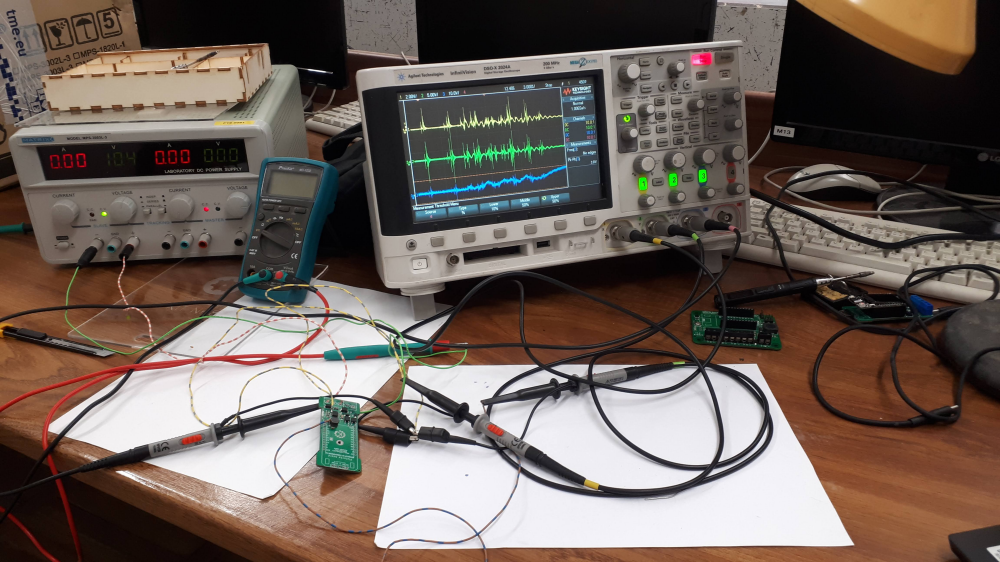
\includegraphics[width=\textwidth]{img/Testovani.png}
    \caption{Testování senzoru}
    \label{fig:SenzorNaStroji}
\end{figure}

%SECTION
\section{Testování ve firmě}
V~bodě kdy byly odladěny chyby jsem systém nasadil na dva pletací stroje.
Nově nasbíraná data byla již reálná a~dalo se na nich postavit nové testování.
Senzory jsem tedy nechal několik dní sbírat údaje o~upletených ponožkách a~následně jsem nad nimi spustil generování uživatelsky čitelných dat.

Od půlky prosince 2020 probíhá dlouhodobé testování bez zásahu do vygenerovaných dat. Naměřené údaje pravidelně stahuji a~kontroluji jejich správnost.

\newpage


\chapter{Nasazení}
Lorem ipsum dolor sit amet, consectetur adipiscing elit.
Aliquam nunc magna, sollicitudin id leo eu, viverra congue risus.
Aliquam consequat ipsum ut erat placerat consequat nec at diam. 
Aenean est odio, molestie sit amet nunc in, pretium luctus elit. 
Donec imperdiet orci vel porttitor placerat. 
Proin ut hendrerit elit, ultricies accumsan urna. 
Vivamus condimentum lorem viverra lectus finibus, nec volutpat turpis auctor.
Cras quis felis non lorem consectetur interdum eu eu sem. 
Proin sit amet feugiat metus. 
Ut vitae orci a enim vestibulum porta. 



%SECTION
\section{Nasazení ve firmě}
Lorem ipsum dolor sit amet, consectetur adipiscing elit.
Aliquam nunc magna, sollicitudin id leo eu, viverra congue risus.
Aliquam consequat ipsum ut erat placerat consequat nec at diam. 
Aenean est odio, molestie sit amet nunc in, pretium luctus elit. 
Donec imperdiet orci vel porttitor placerat. 
Proin ut hendrerit elit, ultricies accumsan urna. 
Vivamus condimentum lorem viverra lectus finibus, nec volutpat turpis auctor.
Cras quis felis non lorem consectetur interdum eu eu sem. 
Proin sit amet feugiat metus. 
Ut vitae orci a enim vestibulum porta. 


\subsection{Zpětná vazba}
Lorem ipsum dolor sit amet, consectetur adipiscing elit.
Aliquam nunc magna, sollicitudin id leo eu, viverra congue risus.
Aliquam consequat ipsum ut erat placerat consequat nec at diam. 
Aenean est odio, molestie sit amet nunc in, pretium luctus elit. 
Donec imperdiet orci vel porttitor placerat. 
Proin ut hendrerit elit, ultricies accumsan urna. 
Vivamus condimentum lorem viverra lectus finibus, nec volutpat turpis auctor.
Cras quis felis non lorem consectetur interdum eu eu sem. 
Proin sit amet feugiat metus. 
Ut vitae orci a enim vestibulum porta. 




\newpage


\chapter*{Závěr}

Cílem této práce bylo navrhnout ucelený systém, který dokáže:

\begin{itemize}
    \item počítat upletené ponožky
    \item zjišťovat poruchovost strojů
    \item porovnávat jednotlivé pracovní směny
    \item monitorovat průběh výroby
\end{itemize}

Všechny tyto vytyčené cíle se mi podařilo splnit. Systém nadále běží ve firmě ROTEX Vysočina s.r.o \cite{ROTEX} a~pomáhá v~běžném provozu.
Můj systém se stal nedílnou součástí výrobního procesu a~analyzuje průběh výroby.

Systém mám k~1. únoru 2021 nasazen na deseti pletacích strojích a~po dobu provozu zaznamenal již přes padesát tisíc upletených ponožek.
Celý systém je nasazený krátkou dobu, abych dokázal porovnat produktivitu před nasazením tohoto systému s~daty po nasazení.

Velkým přínosem pro firmu je porovnávání pracovních směn, díky kterým zaměstnavatel ihned vidí rozdíly mezi produktivitou práce v~daném čase.

Díky SOČ jsem se naučil navrhovat plošné spoje, rozšířil jsem si obzory v~elektronice a při vývoji jsem si vyzkoušel práci s měřícími přístroji. 
Také jsem se naučil programovat v~jazyce PHP a~vytvářet komplexní webové systémy.

V~budoucnu bych chtěl tento systém rozšířit na všechny pletací stroje a~pokrýt tak celou výrobnu.
Taktéž pokračuji na vylepšování webové aplikace a~plánuji ji rozšířit o~další funkce.
Jde například o~export dat do tabulek.

Tuto práci můžete najít na adrese: \url{https://github.com/JakubAndrysek/SOC-Integrace-do-prumyslu-4.0/blob/master/text.pdf}.

Všechny zdrojové kódy a DPS k projektu jsou k dispozici na \url{https://github.com/Pletacka-IoT} pod MIT licencí.


\newpage

\newpage



\appendix
\addcontentsline{toc}{chapter}{Přílohy}


% \chapter{}


\begin{figure}[htbp]
    \centering
    % 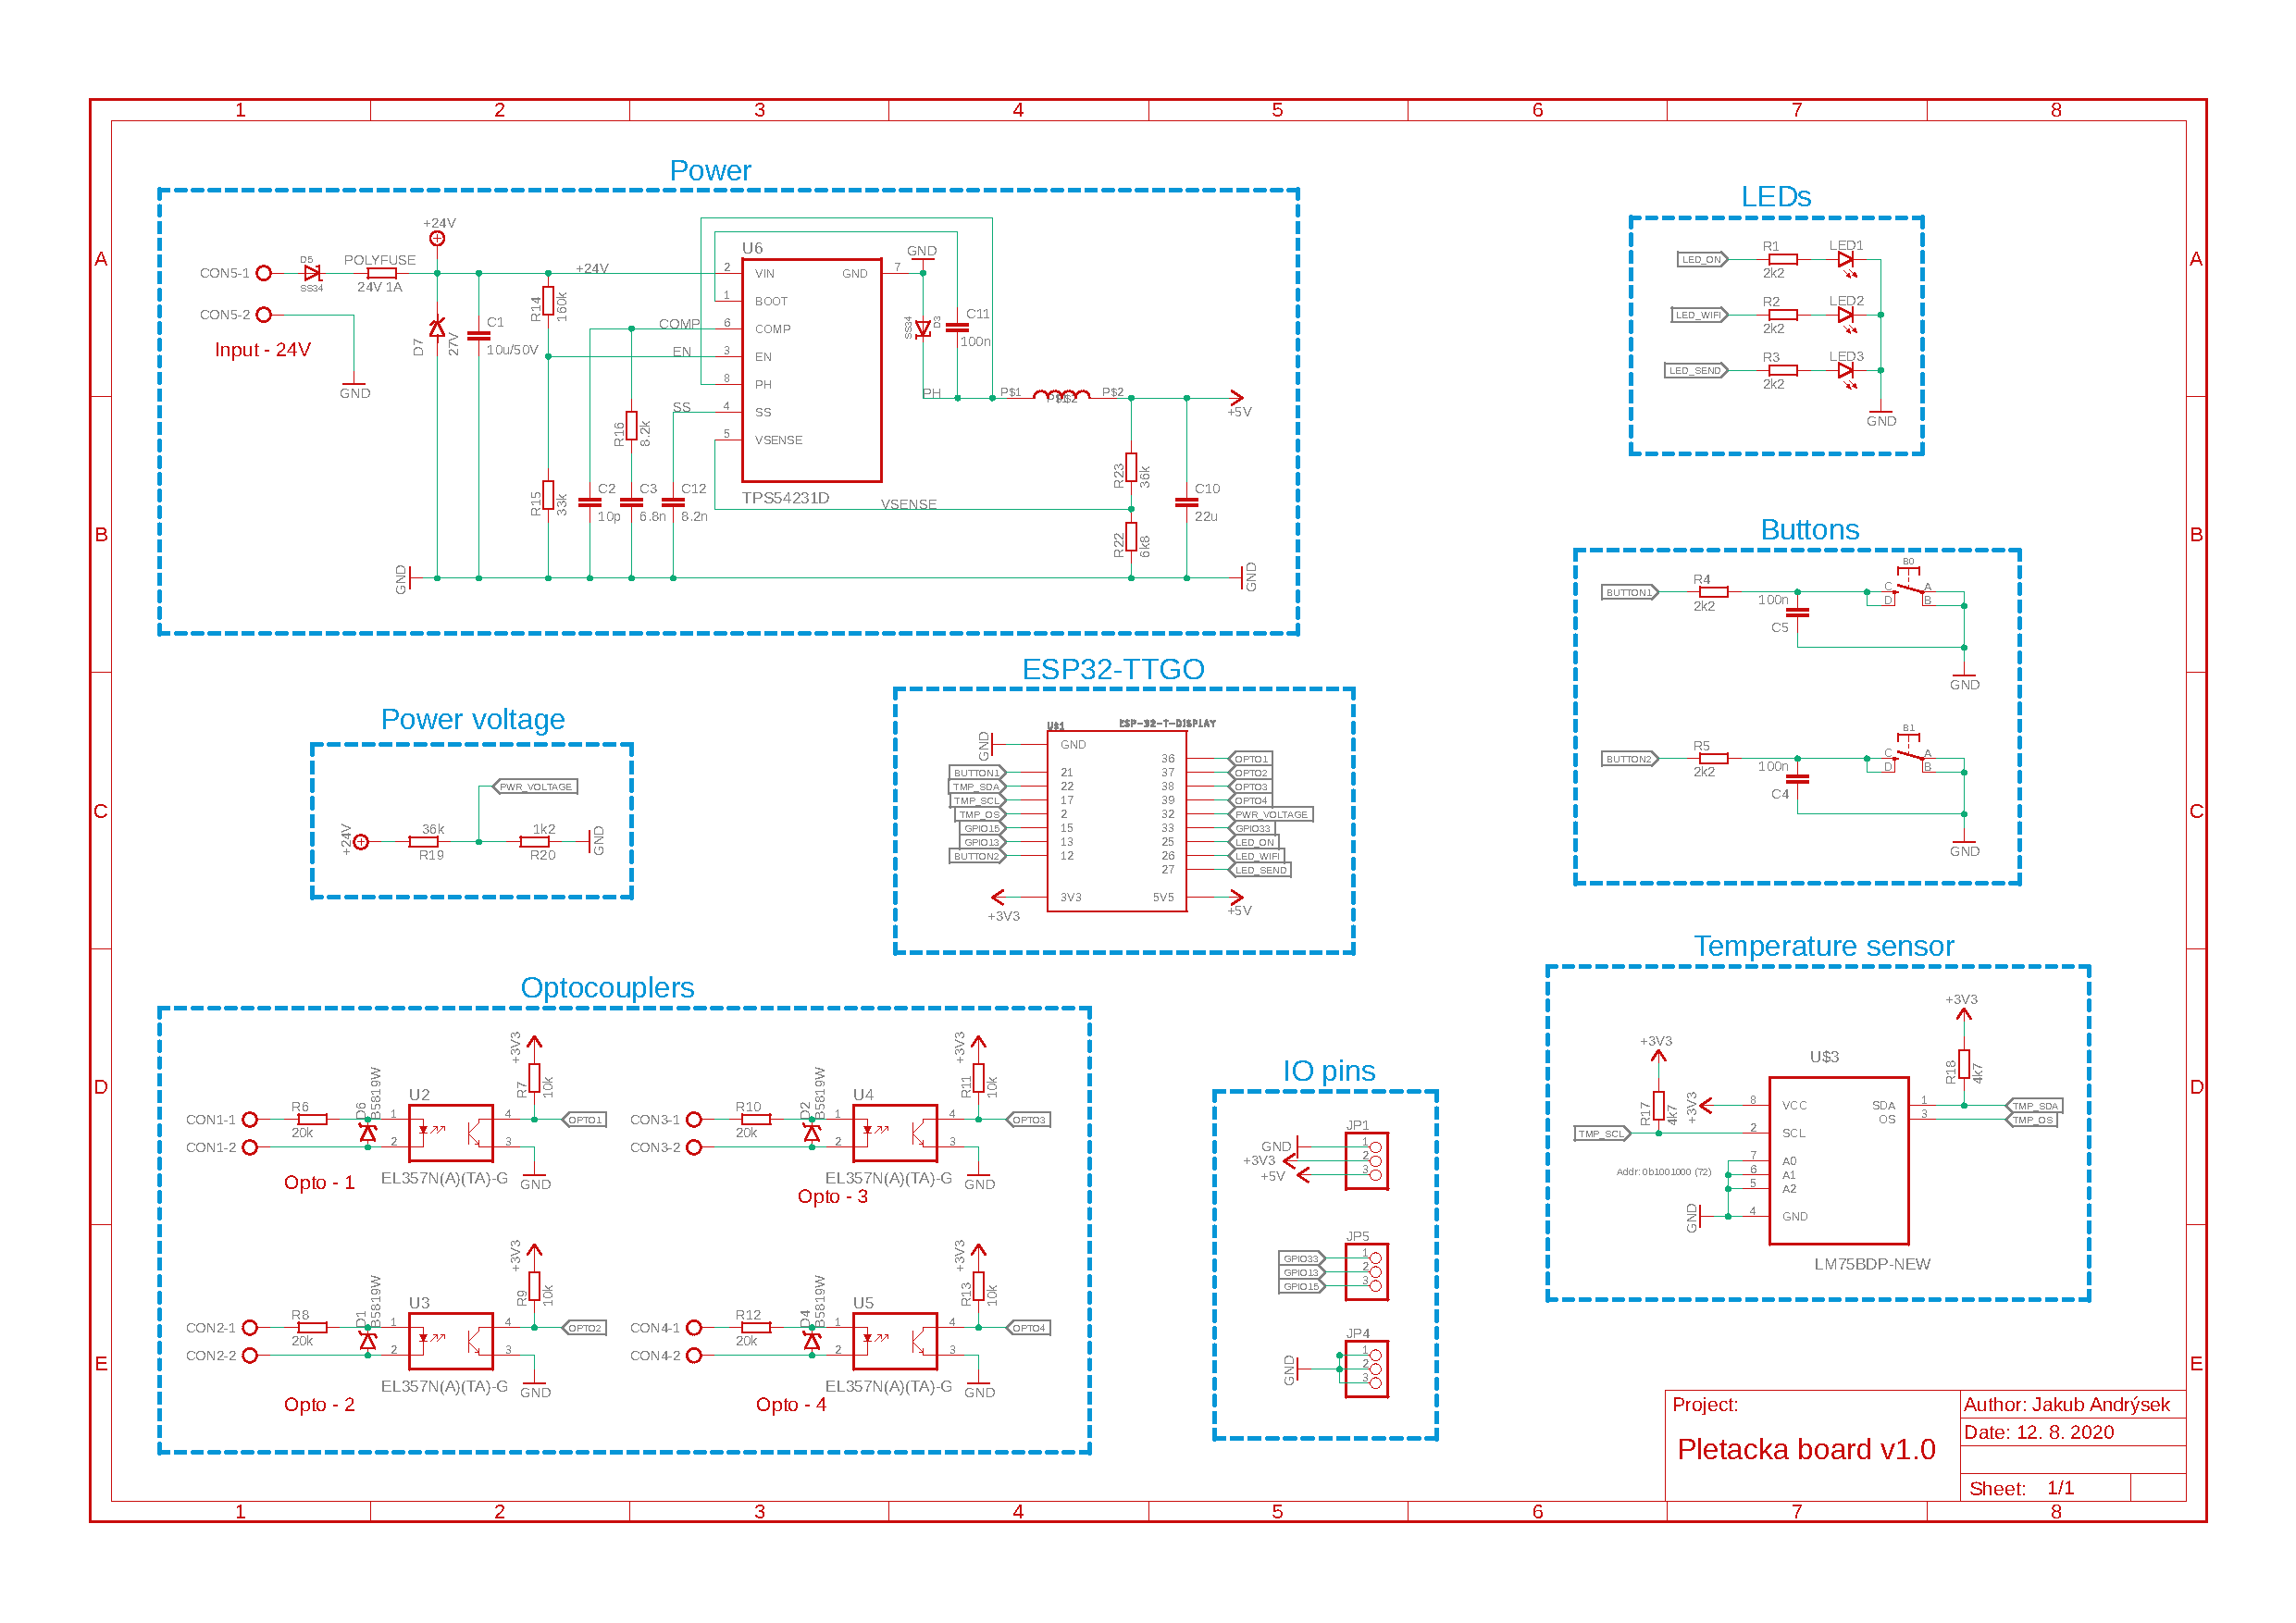
\includegraphics[scale=0.3]{DATASHEET/Pletacka_board_v1.pdf}
    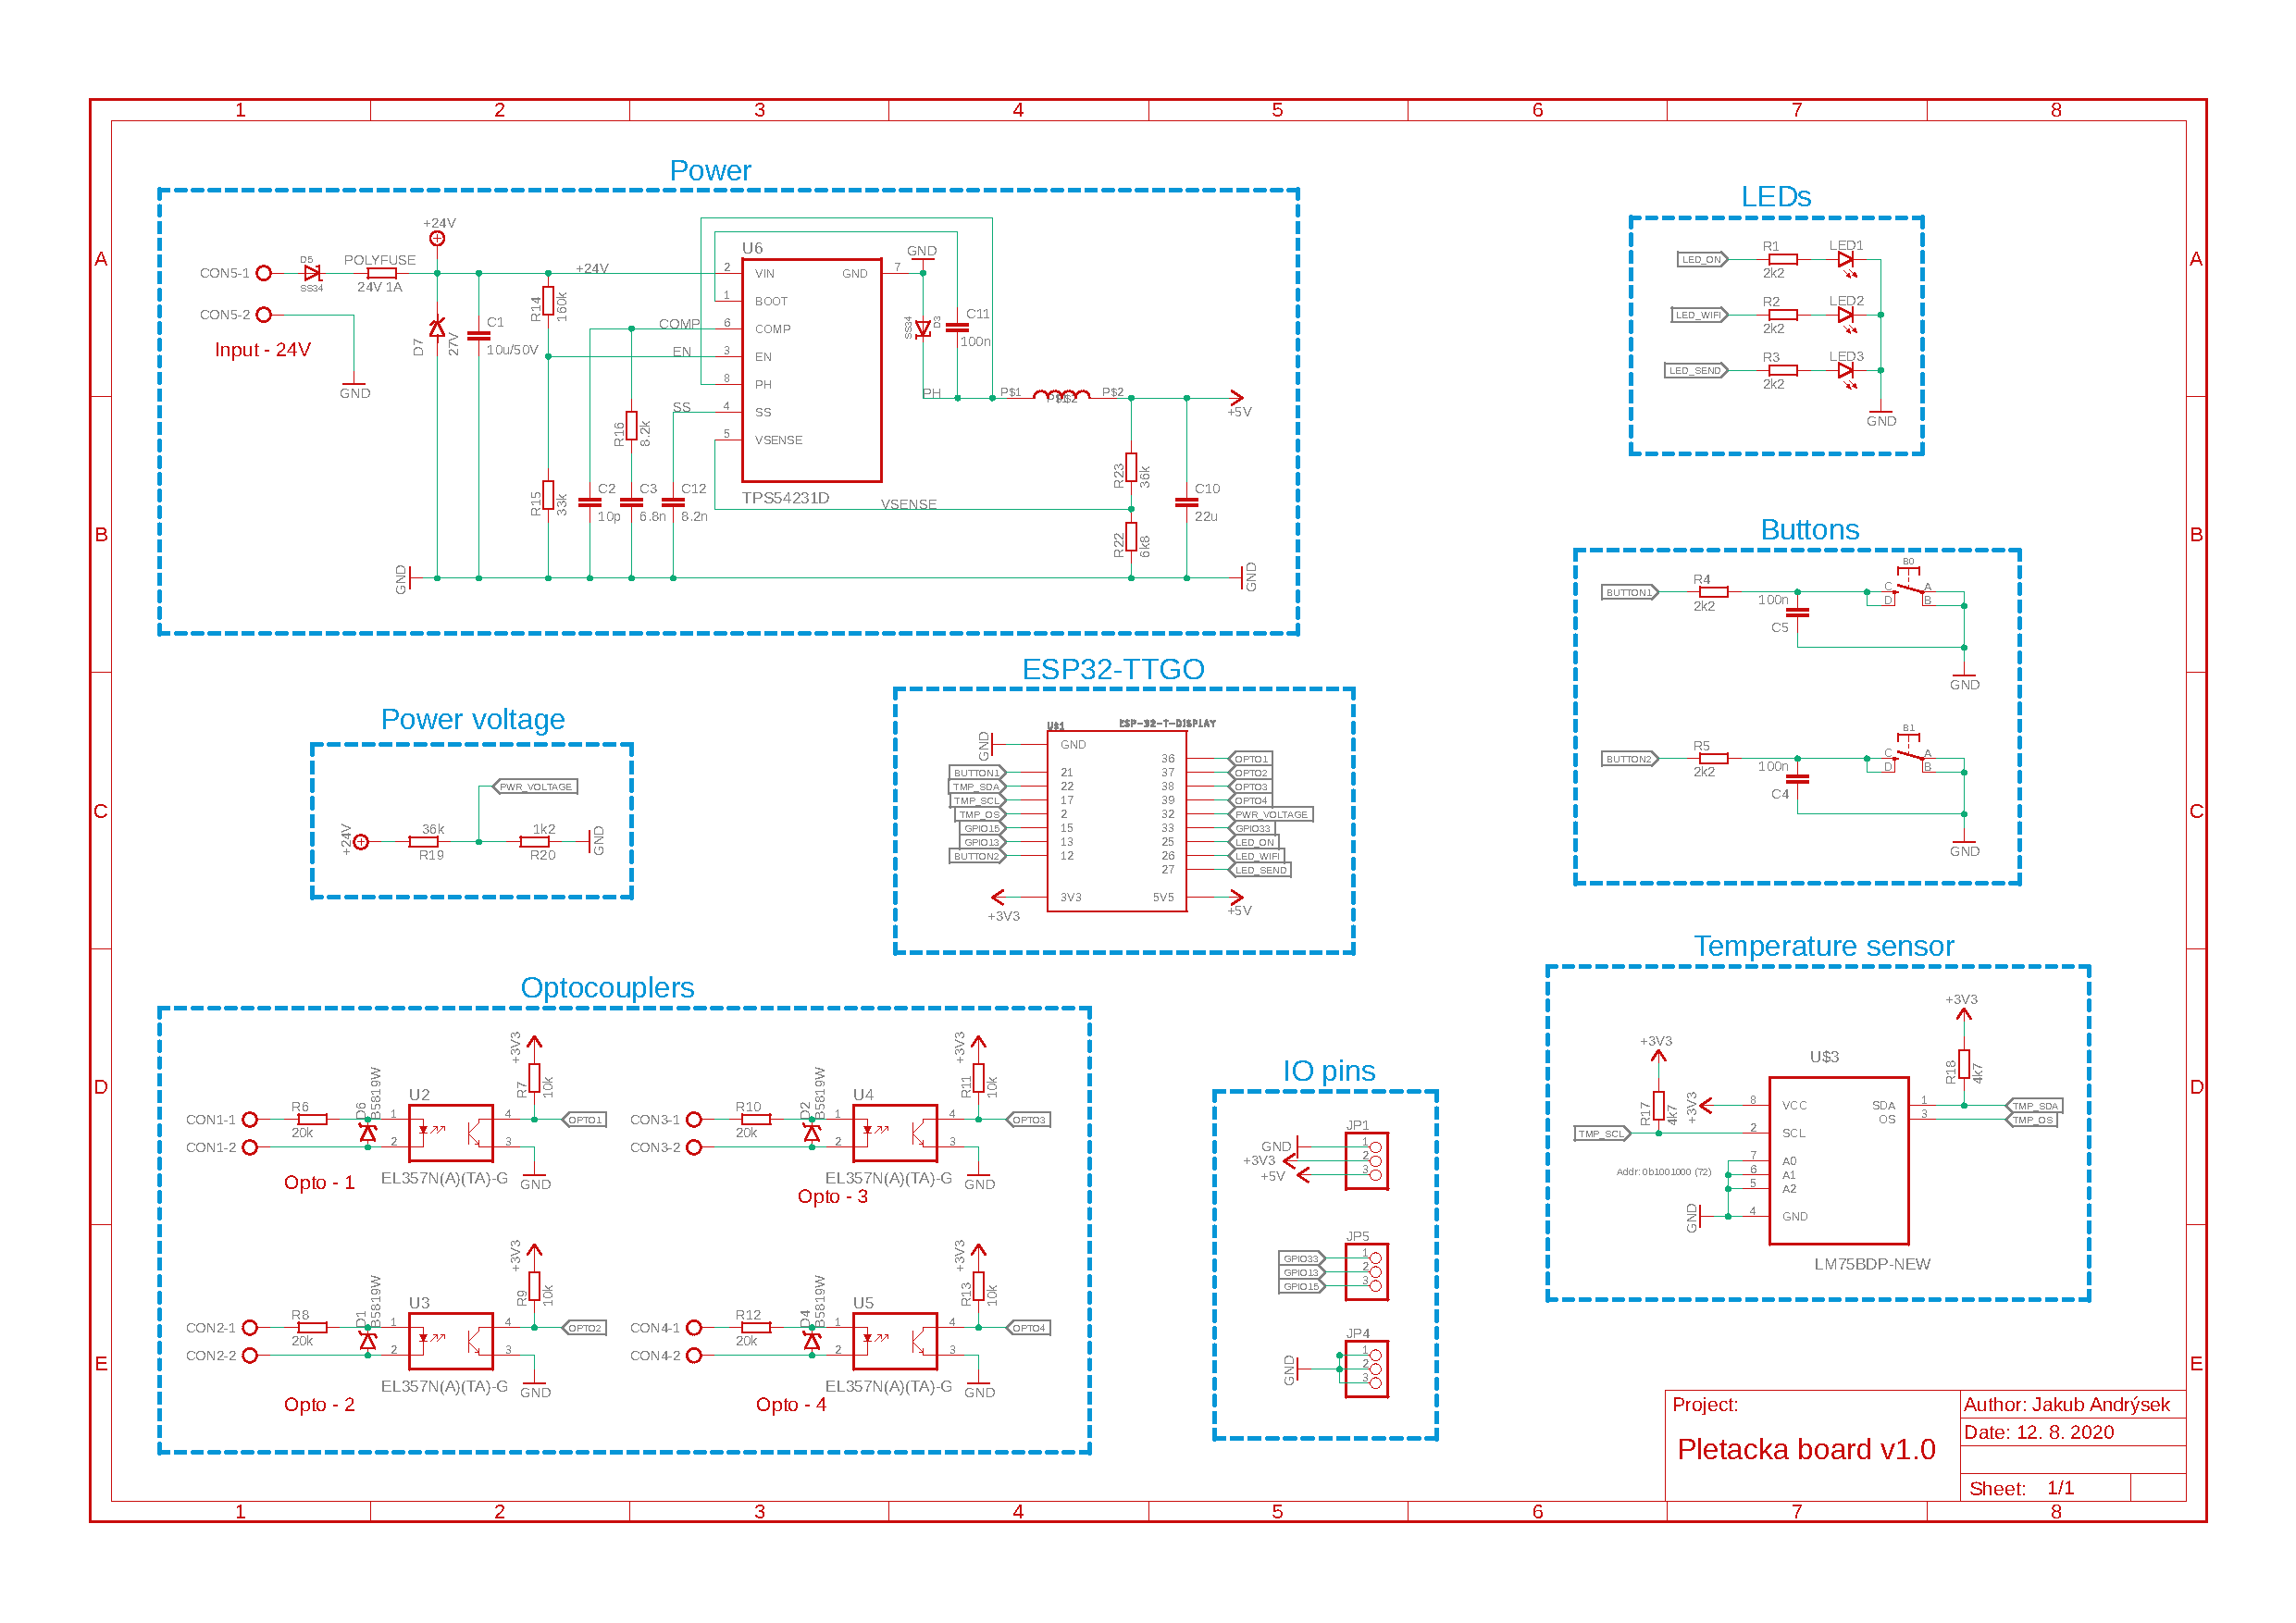
\includegraphics[width=\textwidth]{DATASHEET/Pletacka_board_v1.pdf}
    \caption{Schéma senzoru 1. verze}
    \label{fig:Schemav1}
\end{figure}


\begin{figure}[htbp]
    \centering
    % 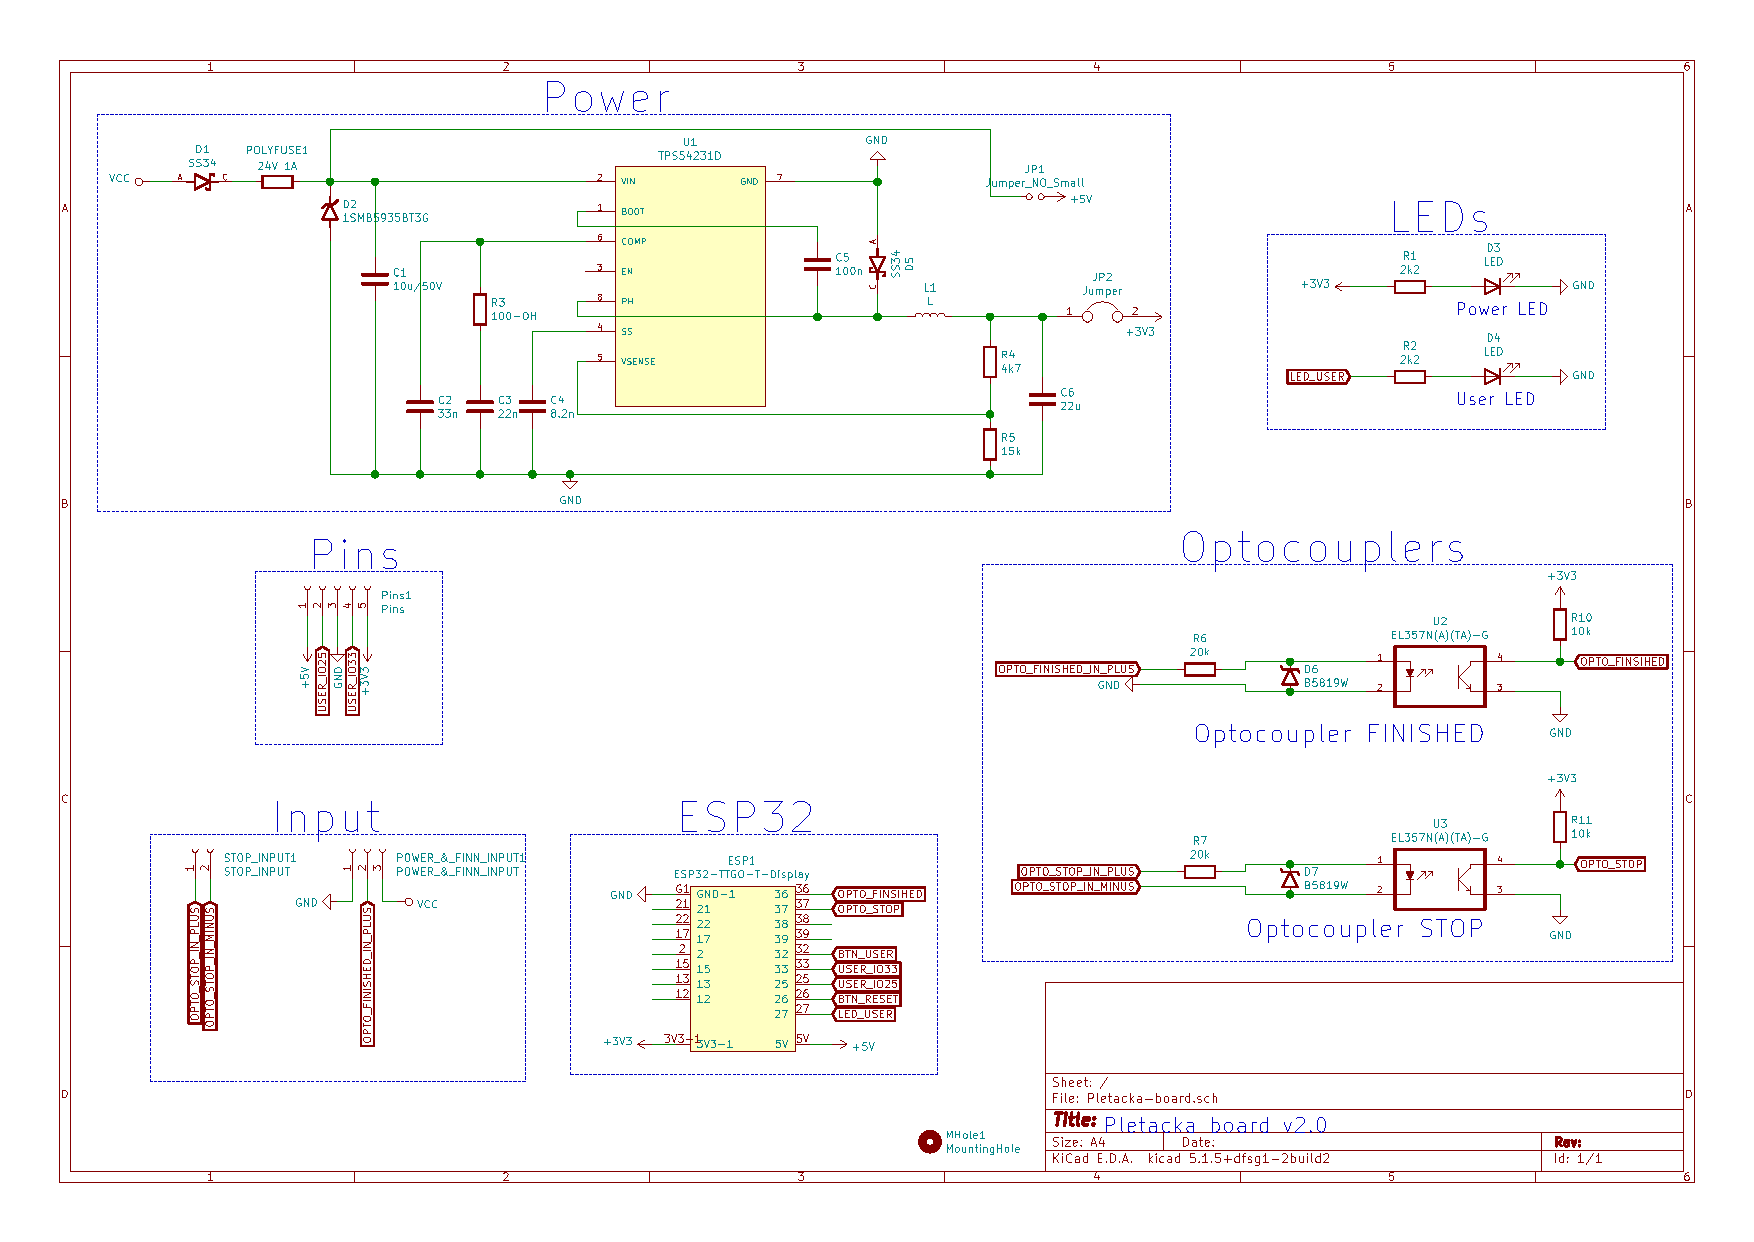
\includegraphics[scale=0.5]{DATASHEET/Pletacka_board_v2.pdf}
    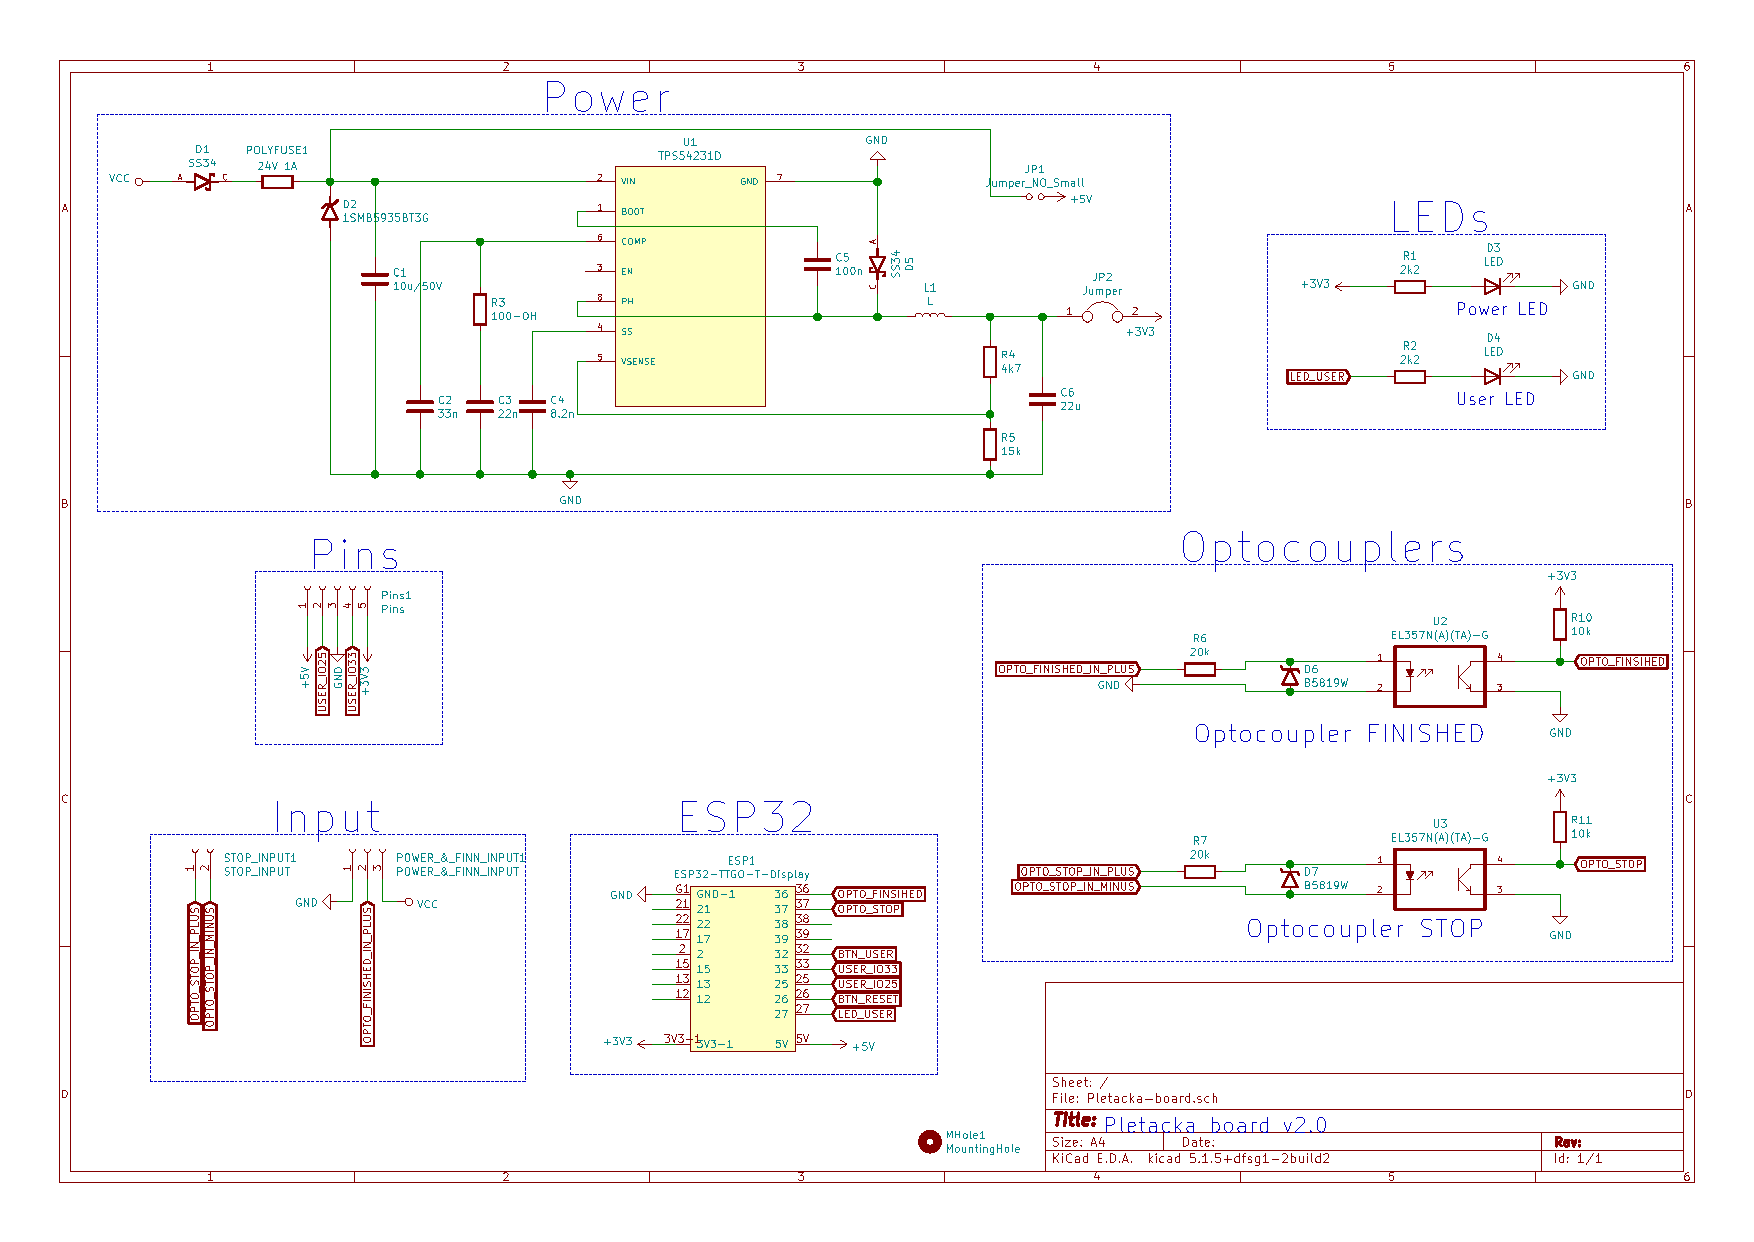
\includegraphics[width=\textwidth]{DATASHEET/Pletacka_board_v2.pdf}
    \caption{Schéma senzoru 2. verze}
    \label{fig:Schemav1}
\end{figure}

\begin{figure}[htbp]
    \centering
    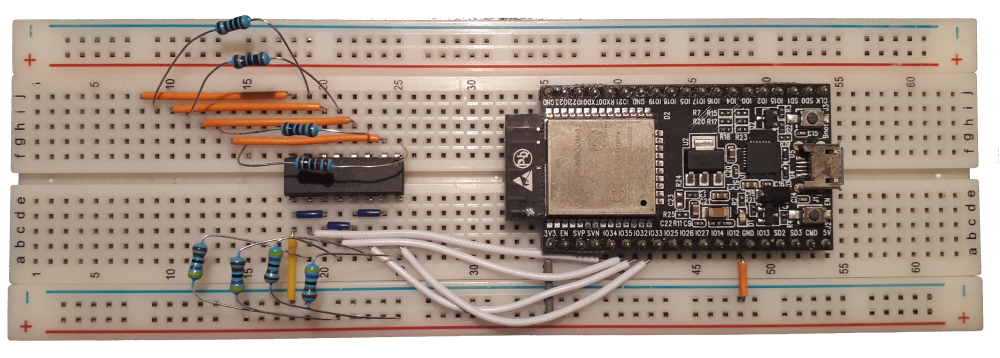
\includegraphics[width=\textwidth]{img/nepajivePole.png}
    \caption{Testování funkčnosti zapojení}
    \label{fig:Pletarna}
\end{figure}


\begin{figure}[htbp]
    \centering
    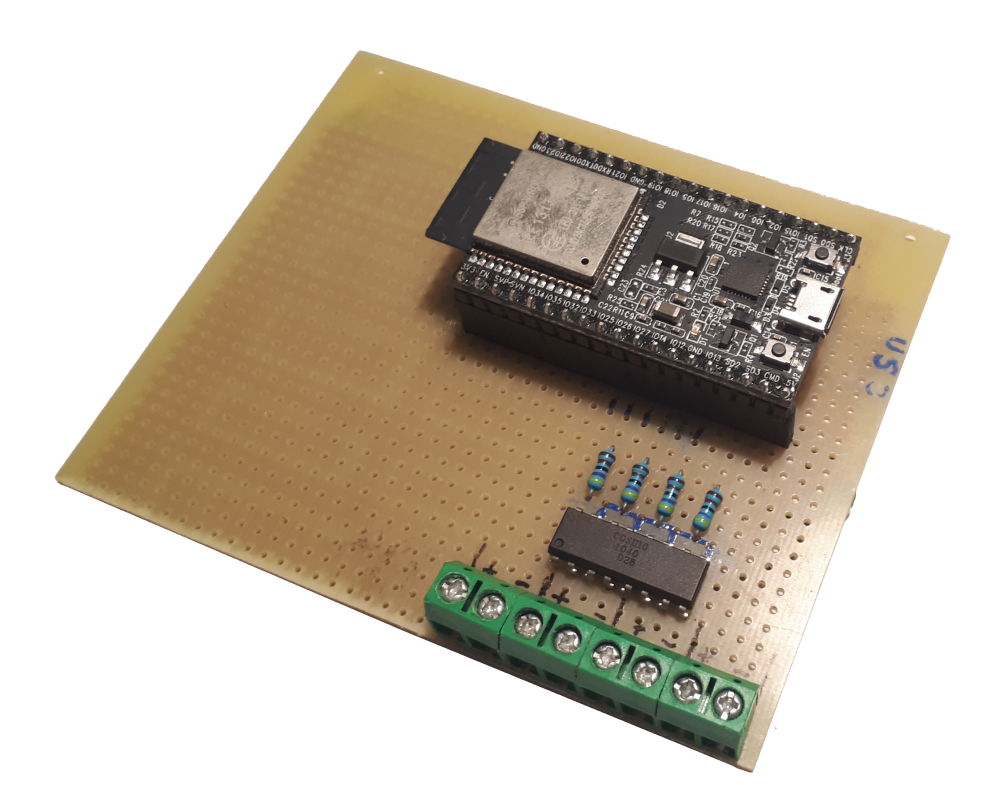
\includegraphics[width=0.8\textwidth]{img/testovaciSenzor.png}
    \caption{Testovací verze senzoru}
    \label{fig:testovaciSenzor}
\end{figure}


\begin{figure}[htbp]
    \centering
    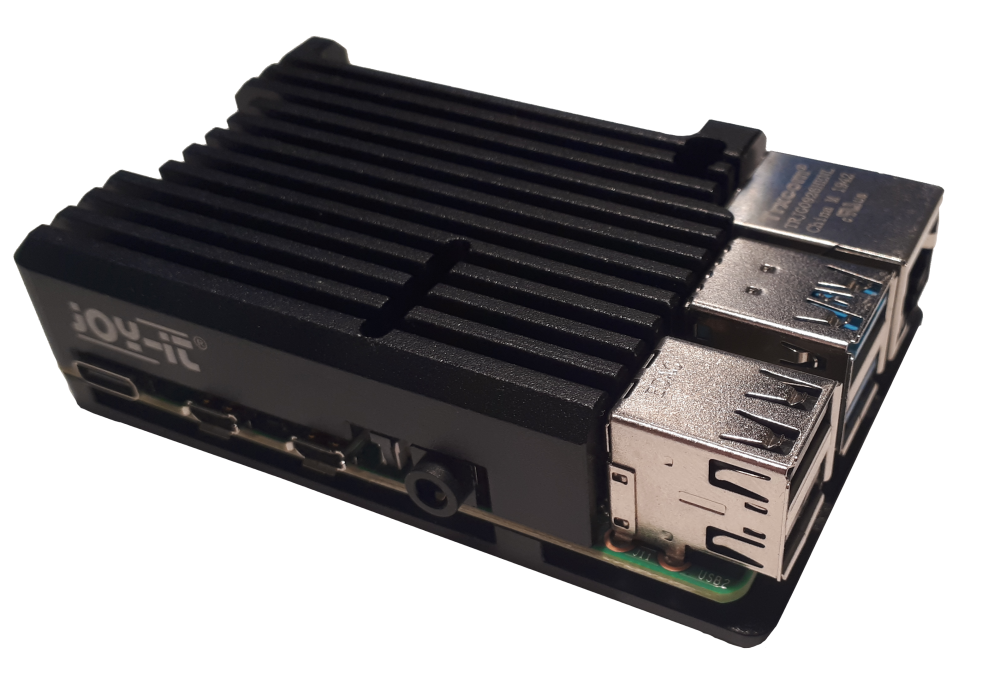
\includegraphics[width=0.8\textwidth]{img/malina.png}
    \caption{Webový server Raspberry Pi}
    \label{fig:malina}
\end{figure}


\begin{figure}[htbp]
    \centering
    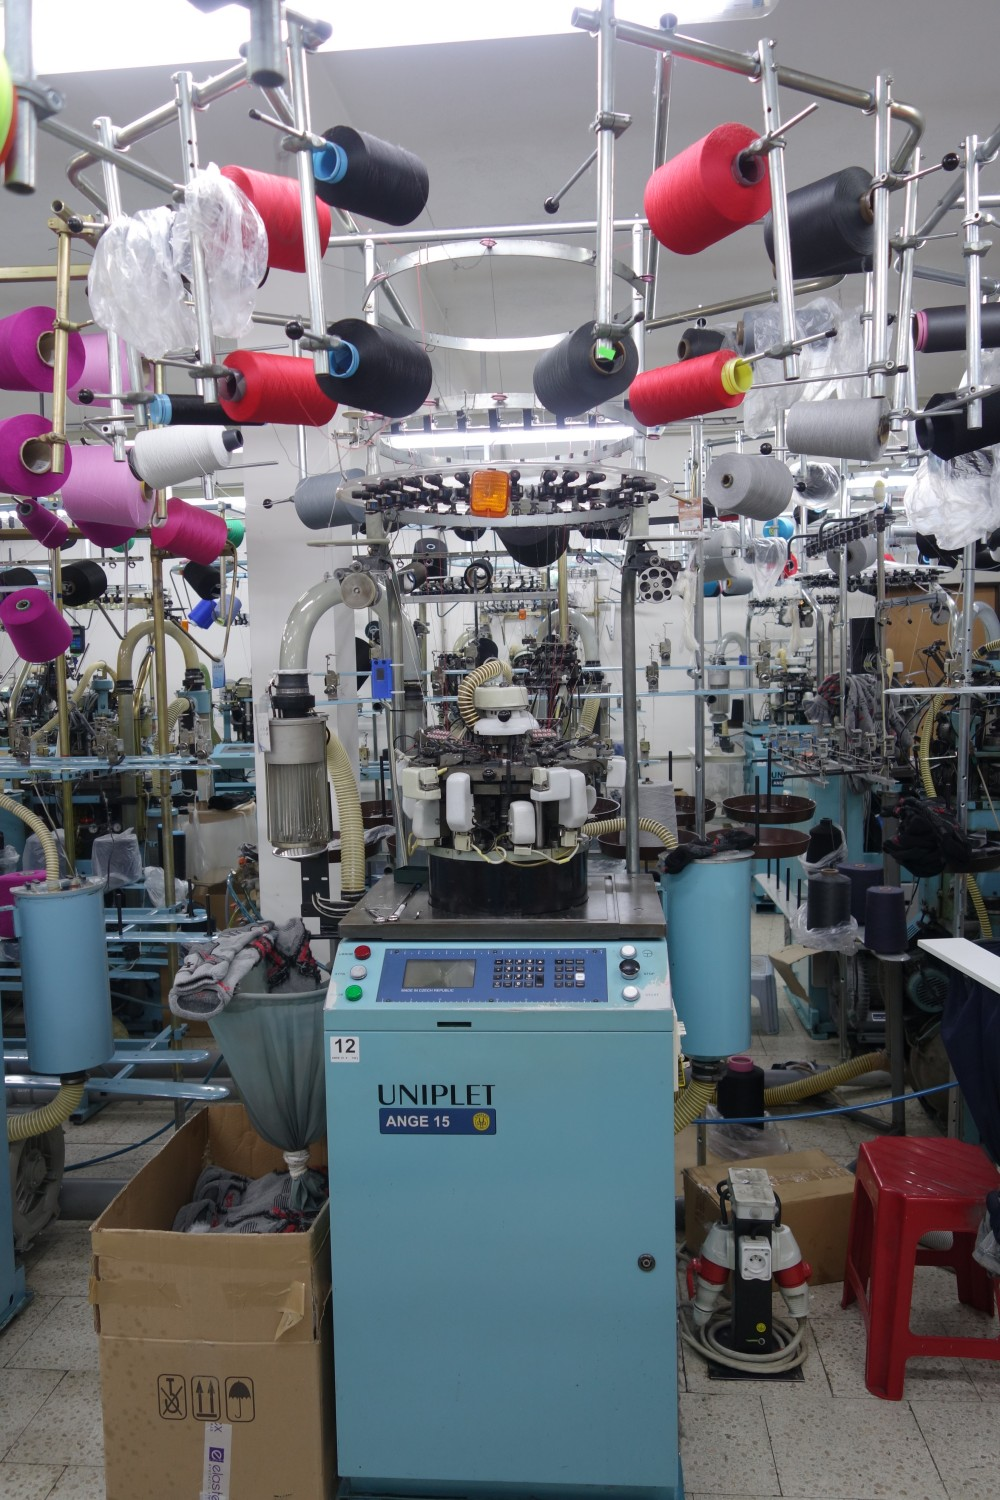
\includegraphics[width=0.9\textwidth]{img/pletacka.png}
    \caption{Pletací stroj}
    \label{fig:pletacka}
\end{figure}

\newpage



\chapter{Senzory}
Lorem ipsum dolor sit amet, consectetur adipiscing elit.
Aliquam nunc magna, sollicitudin id leo eu, viverra congue risus.
Aliquam consequat ipsum ut erat placerat consequat nec at diam. 
Aenean est odio, molestie sit amet nunc in, pretium luctus elit. 
Donec imperdiet orci vel porttitor placerat. 
Proin ut hendrerit elit, ultricies accumsan urna. 
Vivamus condimentum lorem viverra lectus finibus, nec volutpat turpis auctor.
Cras quis felis non lorem consectetur interdum eu eu sem. 
Proin sit amet feugiat metus. 
Ut vitae orci a enim vestibulum porta. 


%SECTION
\section{Pletačka board v1.0}
Lorem ipsum dolor sit amet, consectetur adipiscing elit.
Aliquam nunc magna, sollicitudin id leo eu, viverra congue risus.
Aliquam consequat ipsum ut erat placerat consequat nec at diam. 
Aenean est odio, molestie sit amet nunc in, pretium luctus elit. 
Donec imperdiet orci vel porttitor placerat. 
Proin ut hendrerit elit, ultricies accumsan urna. 
Vivamus condimentum lorem viverra lectus finibus, nec volutpat turpis auctor.
Cras quis felis non lorem consectetur interdum eu eu sem. 
Proin sit amet feugiat metus. 
Ut vitae orci a enim vestibulum porta. 


\subsection{Hardware}
Lorem ipsum dolor sit amet, consectetur adipiscing elit.
Aliquam nunc magna, sollicitudin id leo eu, viverra congue risus.
Aliquam consequat ipsum ut erat placerat consequat nec at diam. 
Aenean est odio, molestie sit amet nunc in, pretium luctus elit. 
Donec imperdiet orci vel porttitor placerat. 
Proin ut hendrerit elit, ultricies accumsan urna. 
Vivamus condimentum lorem viverra lectus finibus, nec volutpat turpis auctor.
Cras quis felis non lorem consectetur interdum eu eu sem. 
Proin sit amet feugiat metus. 
Ut vitae orci a enim vestibulum porta. 


\subsection{Software}
Lorem ipsum dolor sit amet, consectetur adipiscing elit.
Aliquam nunc magna, sollicitudin id leo eu, viverra congue risus.
Aliquam consequat ipsum ut erat placerat consequat nec at diam. 
Aenean est odio, molestie sit amet nunc in, pretium luctus elit. 
Donec imperdiet orci vel porttitor placerat. 
Proin ut hendrerit elit, ultricies accumsan urna. 
Vivamus condimentum lorem viverra lectus finibus, nec volutpat turpis auctor.
Cras quis felis non lorem consectetur interdum eu eu sem. 
Proin sit amet feugiat metus. 
Ut vitae orci a enim vestibulum porta. 



%SECTION
\section{Pletačka board v2.0}
Lorem ipsum dolor sit amet, consectetur adipiscing elit.
Aliquam nunc magna, sollicitudin id leo eu, viverra congue risus.
Aliquam consequat ipsum ut erat placerat consequat nec at diam. 
Aenean est odio, molestie sit amet nunc in, pretium luctus elit. 
Donec imperdiet orci vel porttitor placerat. 
Proin ut hendrerit elit, ultricies accumsan urna. 
Vivamus condimentum lorem viverra lectus finibus, nec volutpat turpis auctor.
Cras quis felis non lorem consectetur interdum eu eu sem. 
Proin sit amet feugiat metus. 
Ut vitae orci a enim vestibulum porta. 


\subsection{Hardware}
Lorem ipsum dolor sit amet, consectetur adipiscing elit.
Aliquam nunc magna, sollicitudin id leo eu, viverra congue risus.
Aliquam consequat ipsum ut erat placerat consequat nec at diam. 
Aenean est odio, molestie sit amet nunc in, pretium luctus elit. 
Donec imperdiet orci vel porttitor placerat. 
Proin ut hendrerit elit, ultricies accumsan urna. 
Vivamus condimentum lorem viverra lectus finibus, nec volutpat turpis auctor.
Cras quis felis non lorem consectetur interdum eu eu sem. 
Proin sit amet feugiat metus. 
Ut vitae orci a enim vestibulum porta. 


\subsection{Software}
Lorem ipsum dolor sit amet, consectetur adipiscing elit.
Aliquam nunc magna, sollicitudin id leo eu, viverra congue risus.
Aliquam consequat ipsum ut erat placerat consequat nec at diam. 
Aenean est odio, molestie sit amet nunc in, pretium luctus elit. 
Donec imperdiet orci vel porttitor placerat. 
Proin ut hendrerit elit, ultricies accumsan urna. 
Vivamus condimentum lorem viverra lectus finibus, nec volutpat turpis auctor.
Cras quis felis non lorem consectetur interdum eu eu sem. 
Proin sit amet feugiat metus. 
Ut vitae orci a enim vestibulum porta. 



\newpage


\chapter{Webový server}

!!!!!  Pletačka website !!!!!

Lorem ipsum dolor sit amet, consectetur adipiscing elit.
Aliquam nunc magna, sollicitudin id leo eu, viverra congue risus.
Aliquam consequat ipsum ut erat placerat consequat nec at diam. 
Aenean est odio, molestie sit amet nunc in, pretium luctus elit. 
Donec imperdiet orci vel porttitor placerat. 
Proin ut hendrerit elit, ultricies accumsan urna. 
Vivamus condimentum lorem viverra lectus finibus, nec volutpat turpis auctor.
Cras quis felis non lorem consectetur interdum eu eu sem. 
Proin sit amet feugiat metus. 
Ut vitae orci a enim vestibulum porta. 



\section{Struktura projektu}
Lorem ipsum dolor sit amet, consectetur adipiscing elit.
Aliquam nunc magna, sollicitudin id leo eu, viverra congue risus.
Aliquam consequat ipsum ut erat placerat consequat nec at diam. 
Aenean est odio, molestie sit amet nunc in, pretium luctus elit. 
Donec imperdiet orci vel porttitor placerat. 
Proin ut hendrerit elit, ultricies accumsan urna. 
Vivamus condimentum lorem viverra lectus finibus, nec volutpat turpis auctor.
Cras quis felis non lorem consectetur interdum eu eu sem. 
Proin sit amet feugiat metus. 
Ut vitae orci a enim vestibulum porta. 

\section{Uživatelské rozhraní}
Lorem ipsum dolor sit amet, consectetur adipiscing elit.
Aliquam nunc magna, sollicitudin id leo eu, viverra congue risus.
Aliquam consequat ipsum ut erat placerat consequat nec at diam. 
Aenean est odio, molestie sit amet nunc in, pretium luctus elit. 
Donec imperdiet orci vel porttitor placerat. 
Proin ut hendrerit elit, ultricies accumsan urna. 
Vivamus condimentum lorem viverra lectus finibus, nec volutpat turpis auctor.
Cras quis felis non lorem consectetur interdum eu eu sem. 
Proin sit amet feugiat metus. 
Ut vitae orci a enim vestibulum porta. 

\section{Backend}
Lorem ipsum dolor sit amet, consectetur adipiscing elit.
Aliquam nunc magna, sollicitudin id leo eu, viverra congue risus.
Aliquam consequat ipsum ut erat placerat consequat nec at diam. 
Aenean est odio, molestie sit amet nunc in, pretium luctus elit. 
Donec imperdiet orci vel porttitor placerat. 
Proin ut hendrerit elit, ultricies accumsan urna. 
Vivamus condimentum lorem viverra lectus finibus, nec volutpat turpis auctor.
Cras quis felis non lorem consectetur interdum eu eu sem. 
Proin sit amet feugiat metus. 
Ut vitae orci a enim vestibulum porta. 

\section{API}
Lorem ipsum dolor sit amet, consectetur adipiscing elit.
Aliquam nunc magna, sollicitudin id leo eu, viverra congue risus.
Aliquam consequat ipsum ut erat placerat consequat nec at diam. 
Aenean est odio, molestie sit amet nunc in, pretium luctus elit. 
Donec imperdiet orci vel porttitor placerat. 
Proin ut hendrerit elit, ultricies accumsan urna. 
Vivamus condimentum lorem viverra lectus finibus, nec volutpat turpis auctor.
Cras quis felis non lorem consectetur interdum eu eu sem. 
Proin sit amet feugiat metus. 
Ut vitae orci a enim vestibulum porta. 


\newpage


\chapter{Podpůrný server}

!!!Pletačka python server!!!!!!
Lorem ipsum dolor sit amet, consectetur adipiscing elit.
Aliquam nunc magna, sollicitudin id leo eu, viverra congue risus.
Aliquam consequat ipsum ut erat placerat consequat nec at diam. 
Aenean est odio, molestie sit amet nunc in, pretium luctus elit. 
Donec imperdiet orci vel porttitor placerat. 
Proin ut hendrerit elit, ultricies accumsan urna. 
Vivamus condimentum lorem viverra lectus finibus, nec volutpat turpis auctor.
Cras quis felis non lorem consectetur interdum eu eu sem. 
Proin sit amet feugiat metus. 
Ut vitae orci a enim vestibulum porta. 



\section{Komunikace se senzory}
Lorem ipsum dolor sit amet, consectetur adipiscing elit.
Aliquam nunc magna, sollicitudin id leo eu, viverra congue risus.
Aliquam consequat ipsum ut erat placerat consequat nec at diam. 
Aenean est odio, molestie sit amet nunc in, pretium luctus elit. 
Donec imperdiet orci vel porttitor placerat. 
Proin ut hendrerit elit, ultricies accumsan urna. 
Vivamus condimentum lorem viverra lectus finibus, nec volutpat turpis auctor.
Cras quis felis non lorem consectetur interdum eu eu sem. 
Proin sit amet feugiat metus. 
Ut vitae orci a enim vestibulum porta. 

\section{Aktualizace senzorů}
Lorem ipsum dolor sit amet, consectetur adipiscing elit.
Aliquam nunc magna, sollicitudin id leo eu, viverra congue risus.
Aliquam consequat ipsum ut erat placerat consequat nec at diam. 
Aenean est odio, molestie sit amet nunc in, pretium luctus elit. 
Donec imperdiet orci vel porttitor placerat. 
Proin ut hendrerit elit, ultricies accumsan urna. 
Vivamus condimentum lorem viverra lectus finibus, nec volutpat turpis auctor.
Cras quis felis non lorem consectetur interdum eu eu sem. 
Proin sit amet feugiat metus. 
Ut vitae orci a enim vestibulum porta. 
orci a enim vestibulum porta. 



\newpage



\printbibliography[title=Literatura]
\addcontentsline{toc}{chapter}{Literatura}

\listoffigures
\addcontentsline{toc}{section}{Seznam obrázků}

\listoftables
\addcontentsline{toc}{section}{Seznam tabulek}

\end{document}
